%!TEX encoding = UTF-8 Unicode
%!TEX root = ./../main.tex
%!TEX TS-program = xelatex

\chapter{SVM} % Main chapter title
\label{cap:cinque}
La tesi è volta ad investigare lo scenario in cui si utilizzi un classificatore come base per costruire un Oracolo. Da quest esigenza nasce la necessità di utilizzare uno dei tradizionali metodi statistici di \textit{machine learning}. Nella fattispecie si deve risolvere un problema di \textbf{classificazione binaria} dato che il modello, una volta avvenuto l'addestramento, ha lo scopo di predire come accettante o rigettante , cioè appartenente o meno ad \ac{L} , il campione sotto esame.\\
Tra i moltissimi metodi statistici esistenti forse i più noti sono \textit{Random Forest, Recurrent Neural Network, Convolutional Neural Network} e \ac{SVM}. Tra questi un metodo che è stato molto utilizzato nell'apprendimento di linguaggi sono delle riadattazioni delle \textit{Reti Neurali Ricorrenti}, che si sono dimostrate adeguate allo scopo. In queste sede si è scelto di usare \ac{SVM} perchè rappresentano un classificatore molto potente, e sebbene esistano dei lavori inerenti il tema [RIFERIMENTO UNIVERSAL KERNEL] non sono stati contestualizzati nell'ambito dell'\textit{active learning} per \ac{IIR} oppure sono limitati all'apprendimento di alcune specifiche classi di linguaggi[RIFERIMENTI PLANAR LANGUAGES and LEARNABILITY E DE LA HIGUERA]

\section{Overview teorica}
Il problema che si tenta di risolvere con le \ac{SVM} , che è la radice da cui nascono anche altri modelli , appare sotto diversi nomi come il compromesso bias-varianza[INSERIRE RIFERIMENTO SE LO METTO IN TESI], controllo della capacità e dell'\textit{overfitting} dei dati, ma l'idea è la stessa: dato un problema di \textbf{apprendimento supervisionato}, cioè con un insieme di addestramento di cardinalità finita che contiene i dati etichettati con la rispettiva classe di appartenenza (il \textit{training set}) , le migliori \textit{performances} di generalizzazione\footnote{Cioè una migliore capacità di predire correttamente la classe di appartenenza di dati mai visti, cioè non contenuti nel \textit{training set}. Per questo motivo si parla di classificazione.} del classificatore saranno ottenute dal raggiungimento del giusto equilibrio tra l'\textit{accuracy} sul training set del classificatore e la capacità del modello. La capacità di un modello di classificazione statistico rappresenta la complessità, la potenza espressiva, la ricchezza piuttosto che la flessibilità della famiglia di funzioni $f(x,\alpha)$:
\begin{equation*}
f : X \to Y \quad \text{con } X=\{x_{1},x_{2},\dots,x_{l}\} 
\end{equation*}
$X$ contiene i campioni e rappresenta il \textit{training set} e $Y$ rappresenta i possibili valori delle etichette di ciascun campione e nel caso di \textbf{classificazione binaria} $Y=\{0,1\}$. Inoltre si parla di famiglia di funzioni perchè \ac{SVM} (come gli altri modelli) ha una serie di iperparametri ,rappresentati da $\alpha$ , che identificano i diversi classificatori\footnote{Classificatore e modello non sono termini interscambiabili. Il modello è rappresentato dalle funzioni $f(x,\alpha)$ con $\alpha$ generico ,un classificatore invece è una singola funzione che si ottiene dal modello per una specifica istanza degli \textit{iperparametri} $\alpha$.}.  Una capacità alta implica che le funzioni $f(x,\alpha)$ sono complesse cioè di alto grado ad esempio: il discorso è analogo a ciò che accade in una feedback-forward con tante unità nascoste. Per il principio del \textit{Rasoio di Occam} [INSERIRE RIFERIMENTO AL CAPITOLO 2 DOVE SI PARLA DEL RASOIO] è bene selezionare il classificatore con la capacità minima che contemporaneamente si adatta ai dati del \textit{training set} ma come si vedrà i due aspetti sono in contrapposizione e sarà necessario trovarne il giusto compromesso. Questo assunto più avanti sarà approfondito e giustificato. Per il momento basti dire che un classificatore con troppa capacità è come un botanista con una memoria fotografica che quando vede un albero mai visto --- cioè appartenente a quello che formalmente viene identificato come \textit{test set} --- conclude che non è un albero perchè ha un numero di foglie diverso dagli alberi visti finora: situazione detta di \textit{overfitting} in cui il classificatore si è adattato esclusivamente ai dati del \textit{training set} ma non generalizza (analogo della rete neurale con troppe unità nascoste rispetto alla cardinalità del \textit{training set}). D'altro canto una macchina con bassa capacità è come il fratello pigro del botanista  che classifica qualunque cosa sia verde come un albero. In nessuno dei due casi si avrà una buona generalizzazione.

\subsection{Rischio Atteso}
Supponiamo di avere $l$ osservazioni nel \textit{training set}. Ogni osservazione è una coppia: un vettore $x_{i} \in \mathbb{R}^{n} \text{ , } i=1,\cdots,l$ e l'etichetta corretta corretta associata $y_{i}$. Per semplicità $y_{i} \in \{-1,1\}$. Si assume che le coppie $(x_i,y_i)$ siano estratte da una distribuzione di probabilità cumulativa (CDF) che si indica con $P(x,y)$,  e con $p(x,y)$ la corrispondente densità di probabilità (PDF).  Supponiamo che il modello sta provando ad imparare il mapping $x_i \to y_i \text{ per } i=1,\dots,l$.  Il modello è definito da una serie di possibili mapping $f(x,\alpha) \text{ tali che } x \to f(x,\alpha) $. Il modello rappresenta la classe di funzioni $f(x,\alpha) $, si parla di classe perchè più funzioni possono essere imparate dal modello cambiando gli \textit{iperparametri} $\alpha$ e fissare $\alpha$ (che possono essere più di uno) per un modello si concretizza in un modello ``trained'', cioè in uno specifico classificatore. Ad esempio se il modello è una rete neurale gli \textit{iperparametri} $\alpha$ sono tipicamente i pesi e il bias. \\ Seguendo il riferimento \cite{Vapnik95}, si può definire il \textbf{rischio atteso} per un classificatore ($\alpha$ fissato) come:
\begin{equation}
\label{eqn:rischioatteso}
R(\alpha) = \int \frac{1}{2} \abs{y-f(x,\alpha)} \, dP(x,y) = \int \frac{1}{2} \abs{y-f(x,\alpha)} \, p(x,y) \, dx \, dy
\end{equation}
Il rischio atteso è anche detto \textbf{true mean error}  dato che è calcolato su tutti i possibili valori di $x$ e $y$ ($X \times Y$) cioè tiene conto di tutte le combinazioni sia sulle coppie nel \textit{training set} sia di tutte quelle mai osservate. Inoltre nell'equazione \eqref{eqn:rischioatteso}  $1/2 \abs{y-f(x,\alpha)}$ è una \textbf{funzione di loss} , ma se ne poteva scegliere un'altra in generale è $V(f(x,\alpha),y)$. La specifica funzione di loss scelta nell'equazione \eqref{eqn:rischioatteso} può assumere solo valori in $\mathbb{B}$. Tuttavia $R(\alpha)$ così definito non è utile in quanto quasi mai si conosce $P(x,y)$ o una sua stima ,allora si definisce il \textbf{rischio empirico} sempre per un classificatore:
\begin{equation*}
R_{emp}(\alpha) = \frac{1}{2l} \sum_{i=1}^{l}\abs{y-f(x_{i},\alpha)}
\end{equation*}
e rappresenta il tasso di errore medio sul \textit{training set}. $R(\alpha) - R_{emp}(\alpha)$ è l'errore di generalizzazione. Si dice che un modello generalizza se
\begin{equation*}
\lim_{ l \to \infty} R(\alpha) - R_{emp}(\alpha) = 0
\end{equation*}   
cioè al crescere degli elementi nel \textit{training set} gli elementi mal predetti nel \textit{test set} diminuiscono. Ma come già detto il rischio atteso non è quasi mai calcolabile per come è stato definito, allora con un'impostazione molto simile al \textit{PAC-learning} introdotto in [INSERIRE RIFERIMENTO TESI DOVE SI PARLA DEL PAC LEARNING] Vapnik ha dimostrato in \cite{Vapnik95}  che:

\begin{align}
  \intertext{Definiti} 
  \eta &\text{ : } 0 \leq \eta \leq 1 \notag \\ 
  h &\text{ : } h > 0 \\
  \upvarepsilon &= \sqrt{\biggl(\frac{h(\log (2l/h) + 1) - \log (\eta/4)}{l}\biggl)}\\ \intertext{allora si ha che:} 
  R&(\alpha) \leq R_{emp}(\alpha) +\upvarepsilon \quad \text{con probabilità }1-\eta \label{eqn:vapnik}
\end{align}

dove $h$ è detta \ac{VC} \textbf{dimension} e $\upvarepsilon$ è detto \textbf{learning rate} o \textbf{\ac{VC}} \textbf{\textit{confidence}}. La \ac{VC} \textit{dimension} è una misura della capacità e sarà approfondita nella sottosezione [INSERIRE RIFERIMENTO SOTTOSEZIONE VC DIMENSION].  $R_{emp}(\alpha) +\upvarepsilon$ è talvolta detto \textbf{\textit{risk bound}} dato che è un limite superiore del rischio atteso $R(\alpha)$.  Il risultato dell'equazione \eqref{eqn:vapnik} ci consente di trovare con probabilità $1-\eta$ il classificatore che minimizza $R_{emp}(\alpha) +\upvarepsilon$. Tuttavia calcolare questo minimo è molto difficile come è spiegato nella sottosezione [INSERIRE RIFERIMENTO SOTTOSEZIONE STRUCTURAL RISK MINIMIZATION]. Prima di parlarne si spiega cosa è la \ac{VC} \textit{dimension}.

\subsection{\textit{VC dimension}}
\label{sub:vcdim}
La \ac{VC} \textit{dimension} è una misura della capacità di un insieme di funzioni $\{f(x,\alpha)\}$ che possono essere apprese da un modello statistico, ed è definita come la cardinalità del più largo insieme di punti che un modello può \textbf{\textit{shatter}}. Per \textit{shatter} si intende che una delle funzioni è in grado di etichettare correttamente i punti o meglio di separare punti (che sarebbero dei campioni, delle osservature) con etichettature diverse. Ci si pone  nel caso della classificazione binaria e si fissa il codominio di $\{f(x,\alpha)\}$  in $\{-1,1\} \forall x,\alpha$.  Se un insieme $X$ di $l$ punti viene etichettato in tutti i $2^l$ possibili modi, e per ognuna delle $2^l$ combinazioni, può essere trovata una funzione (con $\alpha$ specifico cioè un classificatore) dell'insieme $\{f(x,\alpha)\}$ che separa (o assegna) correttamente queste etichette, si dice che l'insieme di punti $X$ è ``\textit{shattered}'' dall'insieme di funzioni. Quindi la \ac{VC} \textit{dimension} dell'insieme di funzioni $\{f(x,\alpha)\}$ è definita come il \textbf{massimo} numero di punti che possono essere ``\textit{shattered}'' da $\{f(x,\alpha)\}$. Si osservi che avere per esempio una \ac{VC} \textit{dimension}  pari a tre significa che esiste almeno un insieme fatto da tre punti che può essere ``\textit{shattered}'', ma non è detto (tipicamente non lo è) che tutti gli insiemi di tre punti lo siano\footnote{In questo caso si può solo concludere che non esiste nessun insieme di quattro punti che è ``\textit{shattered}''}. Si fornisce come esempio il calcolo delle \ac{VC} \textit{dimension} dell'insieme costituito da tutte le rette in $\mathbb{R}^2$ identificate dall'equazione $y = mx + q$ in cui i parametri $\alpha$ sono rappresentati da $m \text{ e } q$. I punti possono essere etichettati positivamente o negativamente, quindi per essere ``\textit{shattered}'' da una retta devono essere separati da quest'ultima in base all'etichettatura. Inoltre si rimarca che i punti possono essere collocati in qualunque maniera, ma una volta collocati le varie etichettature devono essere effettuate mantenendo fissa quella collocazione scelta. Con tre punti, si riesce a trovare una collocazione dei tre punti (qualsiasi tranne tre punti allineati) tale che esiste una retta (valori specifici di $m$ e $q$)  che separari i punti positivi da quelli negativi e si riesce a fare ciò per ciascuna delle $2^{3}=8$ etichettature diverse\footnote{Si noti che in queste 8 etichettature  la collocazione dei 3 punti deve restare costante ma si può scegliere un'altra funzione (retta) da un'etichettatura all'altra} come si può apprezzare in figura \ref{fig:sha}. 
\begin{figure}[htp]
	\centering
	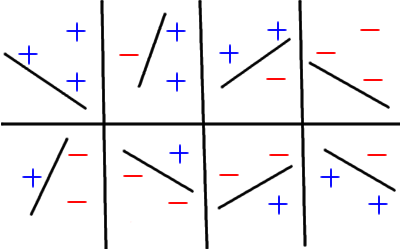
\includegraphics[ width=0.7\textwidth]{RettaShatter}
	\caption[Tre punti shattered nel piano]{Tre punti in $\mathbb{R}^{2}$ , shattered da rette}
   \label{fig:sha}
\end{figure} 

Quattro punti non possono essere ``\textit{shattered}'' quindi la \ac{VC} \textit{dimension} è tre. Più in generale la \ac{VC} \textit{dimension} dell'insieme di iperpiani in $\mathbb{R}^{n}$ è $n+1$. Una dimostrazione di questo risultato si può trovare in \cite[p. 37]{Burges98}. 

\subsection{Structural Risk Minimization}
\label{sub:srm}
La \ac{VC} \textit{dimension} di un modello riveste un ruolo molto importante perchè come si evince dai risultati dell'equazione  \eqref{eqn:vapnik}  ,fissati $\eta \text{ e } l$, si ha che la \ac{VC} \textit{confidence} $\upvarepsilon$ aumenta all'aumentare della \ac{VC} \textit{dimension} $h$. Quindi per diminuire il rischio atteso $R(\alpha)$ sembra sufficiente diminuire $h$ ma in realtà non è così. 
Innanzitutto si precisa che un numero di parametri ($\alpha$) maggiore nel modello non implica  una \ac{VC} \textit{dimension} maggiore infatti esistono dei modelli con un solo parametro e \ac{VC} \textit{dimension} infinita. Inoltre possedere un valore di $h$ più piccolo non comporta necessariamente di avere un rischio atteso più piccolo e quindi un classificatore migliore infatti un valore di $h$ più piccolo significa che è stato ristretto l'insieme delle funzioni $\{f(x,\alpha)\}$ e può accadere che è stata eliminata proprio la funzione che minimizzava il rischio empirico. Quindi dinimuendo $h$ la \ac{VC} \textit{confidence} $\upvarepsilon$ diminuisce ma il rischio empirico può aumentare e quindi diminuire $h$ non implica che il rischio atteso $R(\alpha)$ diminuisca\footnote{Esistono modelli che hanno buoni riscontri pratici nonostante abbiano $h = \infty$}. Il motivo di questo comportamento è che la \ac{VC} \textit{confidence} dipende dalla classe di funzioni $\{f(x,\alpha)\}$ invece il rischio empirico dipende dalla scelta degli \textit{iperparametri} e quindi da una specifica funzione. \\ Al fine di minimizzare $R(\alpha)$ si deve trovare il giusto compromesso tra due quantità che manifestano un andamento opposto al variare di $h$: il rischio empirico (che diminuisce all' aumentare della complessità di  $\{f(x,\alpha)\}$ cioè della capacità del modello cioè all'aumentare di $h$) e la \ac{VC} \textit{confidence} (che diminuisce al diminuire di $h$). Vapnik in \cite{Vapnik82} ha proposto una procedura per affrontare il problema appena delineato detta \ac{SRM} che consiste nel:
\begin{enumerate}
\item Dividere la famiglia di funzioni $\{f(x,\alpha)\}$ in sottoinsiemi autoincludenti come in figura \ref{fig:ssrm} in modo che i sottoinsiemi abbiano una \ac{VC} \textit{dimension} (che è un valore intero) crescente. Ciò significa escludere alcune funzioni da $\{f(x,\alpha)\}$ in modo da trovare la classe di funzioni $h_1$ con \ac{VC} \textit{dimension}  più piccola e così via per $h_{2} \text{,}h_{3}\dots$

\item Per ogni classe di funzioni trovate al punto 1. ($h_{1} \text{,}h_{2}\dots$) trovare quella con il rischio empirico minimo: cioè equivale a una selezione dei parametri. Ad esempio per la classe $h_1$ significa trovare la funzione contenuta in $\{h_{1}(x,\alpha)\}$ che minimizza il rischio empirico (ciè equivale a trovare i parametri $\alpha$ che fanno ciò).

\item Selezionare il classificatore tra quelli trovati al punto 2. che minimizza $R(\alpha)$
\end{enumerate}

\ac{SRM} garantisce un compromesso tra la qualità dell'approssimazione dei dati nel \textit{training set} e la complessità della funzione approssimante come illustrato in figura \ref{fig:srm}

\begin{figure}[htp]
	\centering
	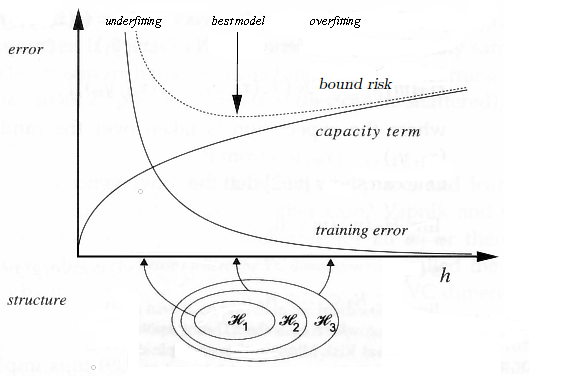
\includegraphics[ width=0.7\textwidth]{SRM}
	\caption[Principio della SRM]{Il \textit{risk bound} è la somma del rischio empirico e la \ac{VC} \textit{confidence}. Il più piccolo \textit{risk bound} è raggiunto su qualche elemento della struttura. }
   \label{fig:srm}
\end{figure} 

\ac{SRM} non è quasi mai applicabile perchè è molto complicato riuscire a calcolare la \ac{VC} \textit{dimension}  delle ``sottofunzioni'' e anche se ciò fosse possibile la difficoltà computazionale per calcolare il rischio empirico , a causa della spesso grande dimensionalità dello spazio degli \textit{iperparametri} del modello, è insostenibile. Si vedrà [INSERIRE RIFERIMENTO DOVE SI PARLA DI COME SVM USI IMPLICITAMENTE SRM,ALALOGO, PER MINIMIZZARE IL RISCHIO ATTESO] che il principio di funzionamento delle \ac{SVM} ricalca concettualmente  da vicino quello della \ac{SRM}.

 \begin{figure}[htp]
	\centering
	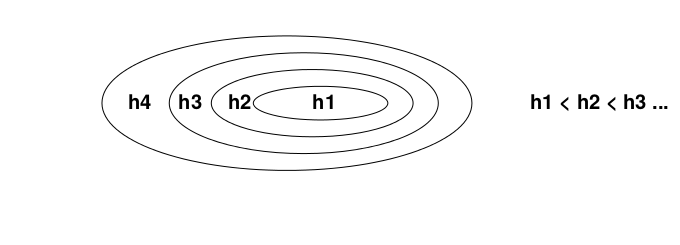
\includegraphics[ width=0.7\textwidth]{SottoinsiemiSRM}
	\caption[Sottoinsiemi \ac{SRM}]{Famiglia di funzioni del modello suddivise in base alla \ac{VC} \textit{dimension} }
   \label{fig:ssrm}
\end{figure}

\section{SVM}
Support Vector Machines (\ac{SVM}) sono un metodo d'apprendimento supervisionato, introdotte per la prima volta da Vapnik e Chervonenkis nel 1963. Nel corso degli anni sono state introdotte varie versioni di \ac{SVM} tra cui ne sono rimarcabili quattro:
\begin{enumerate}
\item Quella originale: Il \textit{Maximal Margin Classifier}.
\item La versione con il \textbf{\textit{kernel}}.
\item La versione detta \textbf{\textit{soft-margin}}.
\item La versione \textit{soft-margin} con \textit{kernel} che combina i tre punti precedenti.
\end{enumerate}
La letteratura sull'argomento è sterminata e \cite{Osuna97} \cite{Burges98} \cite{Ng}  sono solo alcuni dei riferimenti esistenti. Da essi si è tratto gran parte del materiale presentato in questa sezione.
 Le \ac{SVM} consentono di affrontare essenzialmente tre tipi di problemi:
\begin{itemize}
\item Classificazione binaria
\item Classificazione con più classi
\item Regressione lineare
\end{itemize}   

La classificazione binaria è naturale con \ac{SVM} ed è adatta a quei problemi in cui i dati possono appartenere a due classi distinte (etichettate di solito con 1 o -1).\\
Nella classificazione con più classi i dati possono appartenere a più classi.
Nella regressione lineare lo scopo è determinare una funzione lineare che meglio approssimi  un insieme di dati.\\
Il problema affrontato in questa tesi attiene ai problemi di classificazione binaria.

\subsection{Classificazione binaria}
\label{sub:clb}
Un problema di classificazione per molti versi è simile a un problema di inferenza induttiva [INSERIRE RIFERIMENTO TESI]. Da una serie di osservazioni cioè di elementi del \textit{training set} X si deve estrarre il migliore classificatore dallo spazio delle ipotesi $f(x,\alpha)$ secondo qualche criterio di preferenza. Gli elementi del training set in un problema di classificazione binaria supervisionato sono del tipo $(x_i , y_i)$ con $i=1,\dots,l$ cioè $\abs{X}=l$ , $x_i \in \mathbb{R}^{n}$ cioè ogni singolo elemento del \textit{training set} ha dimensionalità $n$, e $y_i \in Y=\{-1,1\}$ (o $\mathbb{B}$ in alcuni casi). La dicotomia delle etichette dell'insieme $Y$ rende la classificazione come \textit{binaria}.
 Nel caso delle \ac{SVM} le funzioni sono del tipo:
\begin{equation*}
f : X \subseteq \mathbb{R}^{n} \to \mathbb{R}
\end{equation*}
Da un punto di vista geometrico la classificazione binaria nelle \ac{SVM} consiste nel trovare l' iperpiano ottimo ,secondo qualche criterio, nello spazio $\mathbb{R}^n$  che separi i dati del \textit{training set} etichettati positivamente da quelli etichettati negativamente. Se almeno un iperpiano siffatto esiste i dati del \textit{training set} sono detti essere \textbf{linearmente separabili}. Un esempio in figura \ref{fig:lsd}\\
Da un punto di vista alanitico è necessario una funzione lineare che classifichi correttamente il \textit{training set}. Una funzione lineare,cioè un iperpiano,  è nella forma:
\begin{equation*}
f(x) = w \bullet x +b = \Biggl(\sum_{i=1}^{n}w_{i}x_{i}\Biggl) + b
\end{equation*}
Quindi la dipendenza dai parametri $\alpha$ si riconduce alla dipendenza da $w$ --- che è un vettore nello spazio $\mathbb{R}^n$ che rappresenta la normale all'iperpiano --- e $b$ uno scalare che consente all'iperpiano di muoversi parallelamente a se stesso.\\  
Una volta scelto il classificatore dallo spazio delle ipotesi, l'ingresso $x=(x_1,x_2,\dots,x_n) $ del \textit{test set} (cioè di un insieme di elementi non sottoposti in fase di addestramento al modello) sarà classificato in base all'esito della funzione $sign(f(x))$ cioè associato alla classe positiva se $f(x) \geq 0$, altrimenti sarà associato alla classe negativa.
 
 \begin{figure}[htp]
	\centering
	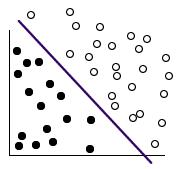
\includegraphics[ width=0.5\textwidth]{linearlyseparabledata}
	\caption[Lineare separabilità]{Dati in $\mathbb{R}^{2}$ linearmente separabili}
   \label{fig:lsd}
\end{figure}

\subsection{Classificatore  a margine massimo}
Il \textit{Maximal Margin Classifier} rappresenta la versione iniziale di \ac{SVM} e spesso in letteratura questa tecnica è nota anche come \textbf{hard margin}. Si applica quando i dati sono \textbf{linearmente separabili}. Come accennato nella sottosezione \ref{sub:clb} è necessario trovare il ``migliore'' iperpiano che separa linearmente i dati nel \textit{training set}. Ai nostri scopi per lineare separabilità si intende che si può trovare una coppia $(w,b)$ tale che i seguenti vincoli sono rispettati:
\begin{align*}
&w \bullet x_i + b \geq \:\:\:1 \quad \quad \qquad\text{ per } y_i = +1 \:\:\:\forall i\\
&w \bullet x_i + b \leq -1 \quad \quad \qquad\text{ per } y_i = -1 \:\:\:\forall i
\end{align*}
I due vincoli possono essere convenientemente combinati insieme in modo da ottenere un unico vincolo più compatto:
\begin{equation}
\label{eq:vin}
y_i(w \bullet x_i + b) - 1 \geq 0 \qquad \qquad \forall i
\end{equation}
Il vincolo \eqref{eq:vin}  deriva dalla constatazione che la \textit{\textbf{decision function}} $sign(w \bullet x + b)$, cioè l'iperpiano separatore ,rispettante il vincolo \eqref{eq:vin}, che viene selezionato come migliore , è tale che se $w$ e $b$ sono scalati\footnote{Per scalati si intende moltiplicati} per la stessa quantità scalare $\alpha \in \mathbb{R}^{+}$  il vincolo \eqref{eq:vin} è ancora rispettato. Dunque per eliminare questa ridondanza , e per rendere ogni \textit{decision function} corrispondente ad un'unica coppia $(w,b)$, viene imposto il seguente vincolo:
\begin{equation}
\label{eq:vin2}
\min_{i=1,\dots,l}^{}\abs{w \bullet x_{i} + b} = 1
\end{equation}
che è un modo equivalente di scrivere il vincolo \eqref{eq:vin}.  Nel gergo tecnico delle \ac{SVM} si suole dire che si è scelto un parametro $\alpha$ tale che il \textit{margine funzionale dell'iperpiano}\footnote{Informalmente il \textit{margine funzionale dell'iperpiano} è la distanza minima tra tutti i punti del \textit{training set} e l'iperpiano separatore} è pari a 1 cioè la valutazione della \textit{\textbf{decision function}} nei punti del \textit{training set}  più vicini all'iperpiano separatore è tale che\footnote{Si può dimostrare che l'esistenza di tali punti è assicurata}
\begin{align}
&w \bullet x_i + b = \:\:\:1 \qquad \qquad\text{ per } y_i = +1 \label{eqn:h1}\\
&w \bullet x_i + b = -1 \qquad \qquad\text{ per } y_i = -1  \label{eqn:h2}
\end{align}
L'nsieme di iperpiani che soddisfano \eqref{eq:vin} sono detti \textbf{Iperpiani Canonici}\footnote{In molte trattazioni si definisce il margine geometrico come il margine funzionale rispetto all'iperpiano normalizzato rispetto a $\norma{w}$ e poi si dimostra che margine funzionale e margine geometrico coincidono imponendo il vincolo  \eqref{eq:vin}}.  Per un'\textit{iperpiano canonico} in cui il margine geometrico e il \textit{margine funzionale dell'iperpiano} coincidono si può dare una definizione intuitiva di \textbf{margine}.
\begin{definizione}
\label{def:mar}
Si indichi con $d_+$ la più breve distanza dell'iperpiano separatore dal più vicino esempio positivo del \textit{training set} e con $d_{-}$ la più breve distanza dall'esempio negativo più vicino del \textit{training set}. Allora:
\begin{equation*}
margine = d_{+} + d_{-}
\end{equation*}
\end{definizione}

Si può dimostrare che la distanza di un punto $x$ da un iperpiano $w \bullet x +b$ è pari a:
\begin{equation*}
d = \frac{\abs{w \bullet x + b}}{\norma{w}}
\end{equation*}
In accordo alla normalizzazione definita in \ref{eq:vin2} la distanza tra l'\textit{iperpiano canonico} e il più vicino degli elementi del \textit{training set} è $\frac{1}{\norma{w}}$. Quindi il margine di un \textit{iperpiano separatore canonico} secondo la definizione \ref{def:mar} è $\frac{2}{\norma{w}}$. L'immagine [INSERIRE RIFERIMENTO IMMAGINE] può essere chiarificatrice.\\

\begin{figure}[htp]
	\centering
	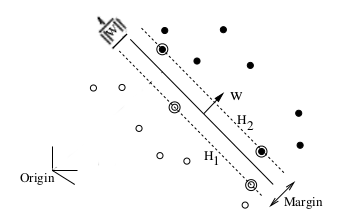
\includegraphics[ width=0.7\textwidth]{Margine}
	\caption[Esempio iperpiano separatore]{Iperpiano separatore per dati linearmente separabili. $H_{1}$ e $H{2}$ sono paralleli dato che hanno la stessa normale $w$ come si apprezza nelle equazioni \ref{eqn:h1} e \ref{eqn:h2}}
   \label{fig:lsd}
\end{figure}

Lo scopo di una \ac{SVM} è:
\begin{enumerate}
\item \label{ite:obj}classificare correttamente il \textit{training set}
\item e selezionare tra quelli che rispettano il punto \ref{ite:obj} quello che generalizza meglio.
\end{enumerate}

Detto succintamente il goal di una \ac{SVM} è trovare l'iperpiano canonico ottimo che separa il \textit{training set} , dove per ottimo si intende quello che massimizza il margine.\\

\subsubsection{Legame con SRM}
In questa sottosezione si vedrà come la tecnica \textbf{hard margin} di \ac{SVM} è in stretta relazione con \ac{SRM} introdotto in [INSERIRE PARTE TESI DOVE  PARLO di SRM]. Si ha infatti che essendo i dati linearmente separabili la rispondenza con il training set è totale quindi $R_{emp}=0$. Quindi il rischio atteso dipende unicamente dalla \ac{VC} \textit{confidence} che a sua volta dipende dalla \ac{VC} \textit{dimension} $h$. Quindi il classificatore migliore nel caso di \ac{SVM} sarà quello con \ac{VC} \textit{dimension} $h$ minima.  La \ac{SRM} in questo caso diventa una ricerca del classificatore con \ac{VC} \textit{dimension} minima. Si consideri inoltre il seguente teorema:
\begin{teorema*}
Sia X un insieme di punti x di uno spazio n-dimensionale  che contiene tutti gli esempi di apprendimento. Sia R il diametro della più piccola ``palla'' (da pensare n-dimesionale) centrata nell'origine che contiene tutti i punti di X. Allora la \ac{VC} dimension ,h, dell'insieme di iperpiani $w \bullet x + b = 0$ aventi margine $\gamma$ è limitata superiormente da: 
\begin{equation*}
h \leq min \biggl( \ceil*{\frac{R^{2}}{\gamma^{2}}} \:\:,\:\: n \biggl) + 1
\end{equation*}
\end{teorema*}
Siccome il margine è $\gamma = 2/\norma{w}$ la \ac{VC} \textit{dimension},h, più piccola (che abbiamo detto minimizza la \ac{VC} \textit{confidence} e avendo il $R_{emp}$ nullo minimizza anche il rischio atteso) si ottiene per la $\norma{w}$ minima cioè per il margine ($2/\norma{w}$) massimo.  Da quanto detto segue che le \ac{SVM} ricercano l'iperpiano col margine massimo per ottenere il classificatore migliore che da cioè più garanzie di generalizzazione secondo il risultato dell'equazione \eqref{eqn:vapnik} e della \ac{SRM}.
Il discorso è analogo ,ma leggermente differente, nel caso in cui i dati non sono linearmente separabili come nel \textbf{soft-margin}[INSERIRE RIFERIMENTO]: in questo caso l'errore empirico non è nullo e le \ac{SVM} cercano per il migliore compromesso tra gli errori nel \textit{training set} e la massimizzazione del margine nell'ottica di minimizzare il \textit{risk boud} $R(\alpha)$.